\section{Conceitos básicos}\label{sec:introducao}

\subsection{Modelos de otimização}\label{subsec:modelos-de-otimizacao}
\begin{frame}
    \frametitle{Modelos de otimização}
    \[
        \min\!/\!\max f(x), x \in \mathcal{X}.
    \]
    \begin{itemize}
        \item $x$: variável de decisão, $x = x_1, x_2, \dots, x_n$.
        \item $\mathcal{X}$: conjunto factível ou domínio;
        \item $f(x)$: função objetivo.
    \end{itemize}
    \note{
        Modelos de otimização são aproximações da realidade, representam o problema de
        maneira simples e objetiva, usando restrições.
        Geralmente quer minimizar ou maximizar uma função $f(x)$ com $x$
        obedecendo algumas restrições.
        \begin{itemize}
            \item $x$: variável de decisão, $x = x_1, x_2, \dots, x_n$.
            \item $\mathcal{X}$: conjunto factível ou domínio,
            possui todas as soluções possíveis para o problema.
            \item $f(x)$: função objetivo, a qual determinará o critério de escolha da solução.
        \end{itemize}
    }
\end{frame}

\subsection{Tipos de soluções}\label{subsec:tipos-de-solucoes}
\begin{frame}
    \frametitle{Tipos de soluções}
    \begin{itemize}
        \item Factível.
        \begin{itemize}
            \item Ótima.
            \item Problema ilimitado.
        \end{itemize}
        \item Problema infactível.
    \end{itemize}
    \note{
        \begin{itemize}
            \item Factível: satisfaz todas as restrições do problema.
            \item Ótima: melhor solução factível.
            \item Problema ilimitado: não é possível encontrar uma solução ótima,
            ou seja, sempre é possível achar uma melhor.
            \item Problema infactível: quando o problema não possui solução,
            geralmente devido a muitas restrições.
        \end{itemize}
    }
\end{frame}

\begin{frame}
    \frametitle{Conceitos básicos}
    \framesubtitle{Modelo contínuo $\times$ discreto}
    \begin{figure}[!htb]
        \centering
        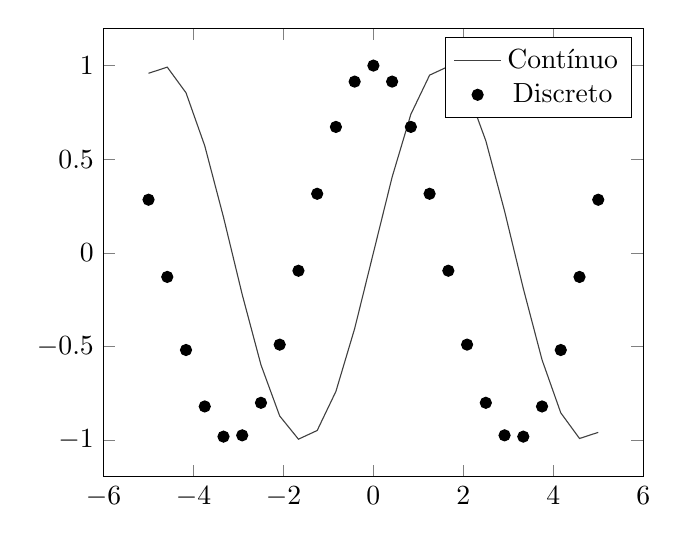
\begin{tikzpicture}
            \begin{axis}
                \addplot[darkgray] {sin((deg(x))};
                \addplot[black, only marks] {cos(deg(x))};
                \legend{Contínuo, Discreto};
            \end{axis}
        \end{tikzpicture}
        \caption{Exemplo de modelo contínuo e discreto.}
        \label{fig:continuo-discreto}
    \end{figure}
    \note{
    % TODO: explicar sobre domínios convexos não convexos
        Um modelo é contínuo quando sua região factível é contínua, ou seja, dado um ponto
        dessa região todos os seus vizinhos também serão uma solução.

        Modelos discretos não possuem seu domínio contínuo.
    }
\end{frame}

\subsection{Métodos exatos × heurísticos}\label{subsec:metodos-exatos-heuristicos}
\begin{frame}
    \frametitle{Métodos exatos × heurísticos}
    \begin{columns}
        \begin{column}{0.5\textwidth}
            Exatos
            \begin{itemize}
                \item Solução ótima.
                \item Tempo.
                \item Recursos.
            \end{itemize}
        \end{column}
        \begin{column}{0.5\textwidth}
            Heurísticos
            \begin{itemize}
                \item Solução factível.
                \item Simplicidade.
                \item Grande porte.
            \end{itemize}
        \end{column}
    \end{columns}
    \note{
        Métodos exatos sempre vão garantir a solução ótima para o problema,
        porém encontrar tal solução pode requerer grande tempo
        e/ou muitos recursos computacionais.

        Já heurísticas buscam por soluções factíveis
        e são geralmente usadas em problemas de grande porte.

        O problema de interesse é NP-difícil, então buscar uma solução ótima fica
        praticamente inviável devido a limitações de tempo e recursos computacionais.
        Uma heurística será utilizada para obter uma solução boa em tempo hábil.
    }
\end{frame}
